%---------------------------------------------------------------------------%
%->> Section 2.2: 大语言模型与智能体应用开发框架
%---------------------------------------------------------------------------%

\section{大语言模型与智能体应用开发框架}

大语言模型（Large Language Model，LLM）是 Transformer 架构~\cite{vaswani2017attention}构建的深度学习模型。它通过大规模预训练获得通用语言表示，并在此基础上展现出对自然语言指令的理解能力。以 GPT 系列~\cite{openai2023gpt4}和 Qwen 系列~\cite{qwen2023technical}为代表的模型，在参数规模扩大后展现出较强的指令跟随、少样本学习和链式推理能力~\cite{wei2022chain}。因此，LLM 开始被用于承担复杂任务中的理解、规划与决策，逐步从语言生成工具转变为任务执行的核心推理引擎。

智能体（Agent）通常指能够感知环境、规划行动并执行操作以完成目标的系统~\cite{yao2022react}。在当前主流实现中，LLM 常作为核心推理引擎，负责理解任务意图、生成执行策略并协调任务流程。感知模块提供环境状态，执行模块负责具体操作，工具模块用于扩展外部信息获取和任务执行能力~\cite{hong2023metagpt}。相较于依赖显式规则的传统软件，这类系统更适合处理开放式任务，尤其是需要多步推进且中间状态难以预先枚举的任务。

从能力构成看，典型智能体系统通常包括记忆、规划、行动和工具使用四个部分~\cite{hong2023metagpt}。如图\ref{fig:agent-system-overview}所示，语言模型作为控制中心与这四类能力持续交互，还可进一步加入反思能力和多智能体协作~\cite{weng2023agent}。其中，记忆用于保存中间结果和历史状态，以支持跨步骤的上下文延续；规划负责分解任务并调整策略；行动负责执行 API 调用、数据库访问或代码操作。工具使用则让模型能够访问外部系统和实时信息，从而突破预训练知识的时效性限制。

\begin{figure}[htbp]
\centering
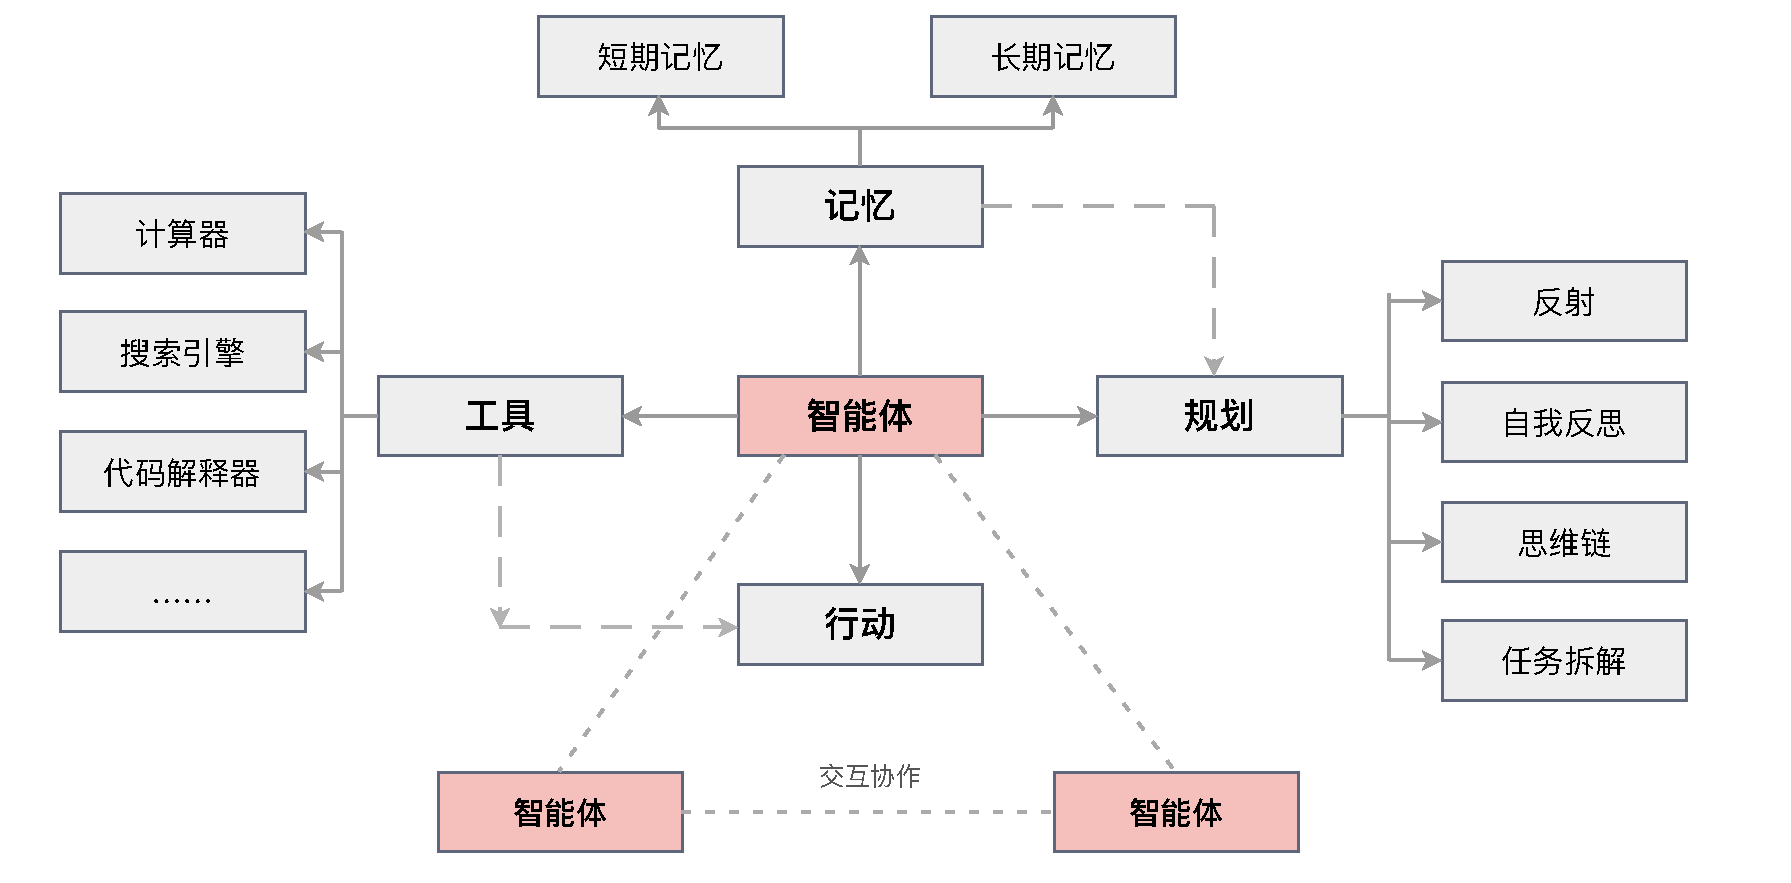
\includegraphics[width=0.95\textwidth]{Figures-Src/Chap2-RelatedWork/Agent/chart.pdf}
\bicaption{\enspace 智能体系统的典型组成（改绘自Weng~\cite{weng2023agent}）}{\enspace Typical Components of an Autonomous Agent System (Redrawn from Weng~\cite{weng2023agent})}
\label{fig:agent-system-overview}
\end{figure}

围绕智能体开发，业界已经形成两类常见支撑环境。一类是通用编排框架。LangChain 提供组件化构建方式，可将多个处理环节组织为链式结构~\cite{langchain}；LangGraph 在此基础上引入状态图机制，以支持更复杂的控制流和状态管理~\cite{langgraph}；Dify 则通过可视化界面配置工作流~\cite{dify}。这类框架更适合流程相对稳定、交互边界较清晰的任务，但在需要频繁调整执行路径的场景中灵活性受限。

另一类是面向真实执行场景的 AI 编程智能体环境。GitHub Copilot~\cite{copilot2024}和 Cursor~\cite{cursor2024}先后把代码补全、多文件问答和重构能力引入开发流程。进一步地，OpenAI Codex~\cite{codex2024}、OpenCode~\cite{opencode2025}、OpenClaw~\cite{openclaw2025}、Google Gemini CLI~\cite{gemini_cli2024}、阿里云 Qwen Code~\cite{qwen_code2025}和 Anthropic Claude Code~\cite{claudecode2024}将文件读写、命令执行和工具调用整合到统一环境中，使模型能够直接操作工程上下文，而不再局限于生成代码片段。

